\documentclass[tikz]{standalone}

\usepackage{fontspec}
\usepackage{amsmath}
\usetikzlibrary{calc}

\begin{document}
    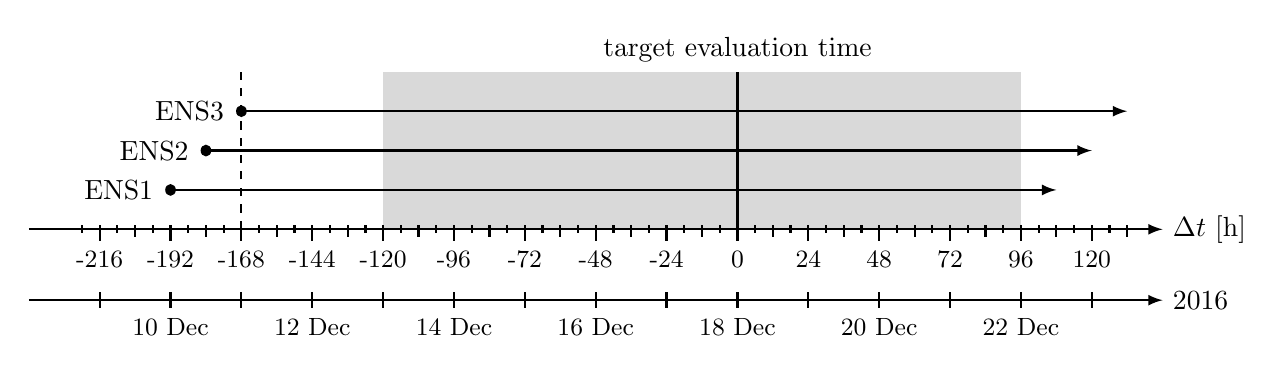
\begin{tikzpicture}[xscale=0.45,yscale=0.5]
        % No-data zones
        \fill[black!15!white] (4,0) rectangle (22,4);
        % Forecasts
        \foreach \x in {1,2,3} {
            \draw[thick,-latex] (\x-3,\x) -- (\x+22,\x);
            \fill[black] (\x-3,\x) circle (0.15) node[anchor=east] {ENS\x\;};
        }
        % Last initial and target evaluation time
        \draw[thick,dashed] (0,0) -- (0,4);
        \draw[thick] (14,0) -- (14,4) node[anchor=south] {target evaluation time};
        % Relative time axis
        \draw[thick,-latex] (-6,0) -- (26,0) node[anchor=west] {$\Delta t$ [h]};
        \foreach \x in {-216,-192,...,120} {
            \draw[thick] (\x/12+13.5,0.1) -- (\x/12+13.5,-0.1);
            \draw[thick] (\x/12+14  ,0.1) -- (\x/12+14  ,-0.3) node[anchor=north,align=center] {\small \x};
            \draw[thick] (\x/12+14.5,0.1) -- (\x/12+14.5,-0.1);
            \draw[thick] (\x/12+15  ,0.1) -- (\x/12+15  ,-0.2);
        }
        % Calendar time axis
        \draw[thick,-latex] (-6,-1.8) -- (26,-1.8) node[anchor=west] {2016};
        \draw[thick] (-4,-1.6) -- (-4,-2.0);
        \foreach \x in {10,12,...,22} { 
            \draw[thick] (2*\x-22,-1.6) -- (2*\x-22,-2.0) node[anchor=north,align=center] {\small {\x} Dec};
            \draw[thick] (2*\x-20,-1.6) -- (2*\x-20,-2.0);
        }
    \end{tikzpicture}
\end{document}

